\chapter{\bevezetes}

Nagyjából egy évvel ezelőtt csatlakoztam a KBPR kollégiumi öntevékeny körbe. A kör végezteti el a kollégium szinte minden nyomtatási munkáját különböző partnerek nyomtatóin, többek közt egy Canon imagePROGRAF PRO-4600 plotteren. Papírtekercsekre nyomtatunk, viszont a kinyomtatott dokumentumok nem mindig tekercs szélességűek. Ez kimondottan gyakori eset, hisz a legtöbb esetben A4-es méretekben nyomtatunk csak vastagabb, minőségibb papírra. Ilyen esetekre szolgált egy \href{fig:old_ui}{Adobe Photoshop script}, ami megpróbálta úgy elrendezni a megadott dokumentumokat, hogy azok egy tekercs szélességű rácson a lehető legkevesebb papírfelesleggel helyezkedjenek el, majd hozzáadott segédvonalakat, amik mentén később a kívánt méretre lehet vágni a kinyomtatott papírt.

Ez a script több hallgató keze műve volt, más-más verziói különböző funkcionalitást voltak képtelenek megvalósítani. Több sebből vérzett, de a legkevésbé sem tudom emiatt az eredeti szerzőit hibáztatni - a scriptet egy évvel ezelőtt erőteljesen refaktoráltam, és saját magam is szembesültem az Adobe ExtendScript nehézségeivel. A projekt nyílt forráskódú és a \href{https://github.com/SCH-KB-PR/kbpr-ps}{https://github.com/SCH-KB-PR/kbpr-ps} oldalon érhető el.

Felmerült az is, hogy keressünk már létező, erre specializálódó szoftvert. A plotterünk cseréje után erre sor is került, ugyanis járt mellé több különböző hivatalos Canon szoftver, azonban egyikük sem felelt meg a céljainknak, hasonlóképp mindegyikből hiányzott egy-egy funkció, amire szükségünk volt, nem beszélve arról, hogy hasonlóképp lassúak és nehezen használhatóak voltak, és hogy kizárólag Windows operációs rendszer alatt működnek.

A script egy nagy erőlelépést jelentett, és gyorsan áttértünk a használatára. Azonban nem volt tökéletes, főként a Photoshop hatalmas overheadje miatt: a dokumentumok generálása sokáig tartott, és volt, hogy a rendelkezésre álló 8 GB ram sem volt elég. Ezeket a program script jellegéből adódóan nem volt lehetőségem tovább optimalizálni, ezért döntöttem úgy, hogy elkészítek egy hasonló programot, ami már a kezdetektől fogva törekszik az optimalizációra. Felmerült továbbá az az ötlet is, hogy tudjunk különböző méretű képeket egyszerre nyomtatni, erről még később bővebben lesz szó.

Az ötlet még 2024 végén érkezett, amikor egy közös szoftverfejlesztési projektet szerettünk volna egy barátommal, Orbán Levente Lászlóval. Eleinte nem volt szilárd elképzelésünk, viszont annyi biztos volt, hogy nyílt forráskóduvá és elsősorban Linux operációs rendszert támogató programot szeretnénk közösen készíteni, ahol a nyelvi elemek terén ő tudna engem, a tervezés terén pedig én tudnám őt mentorálni. Az ő hozzájárulásával választottam az akkor még éppen alig elkezdett projektet az önálló laboratóriumom témájának, és a munkáját részletezni fogom.

\break

A továbbiakban szeretnék részletesebben kitérni a program specifikációjára, a rendszer tervére, annak megvalósítására és a felmerült nehézségekre, majd a szoftver tesztelésre, értékelésére, végül a projekt jövőjére. Mellékletként egy rövid felhasználói kézikönyvet is fogok csatolni.

\begin{figure}[h]
    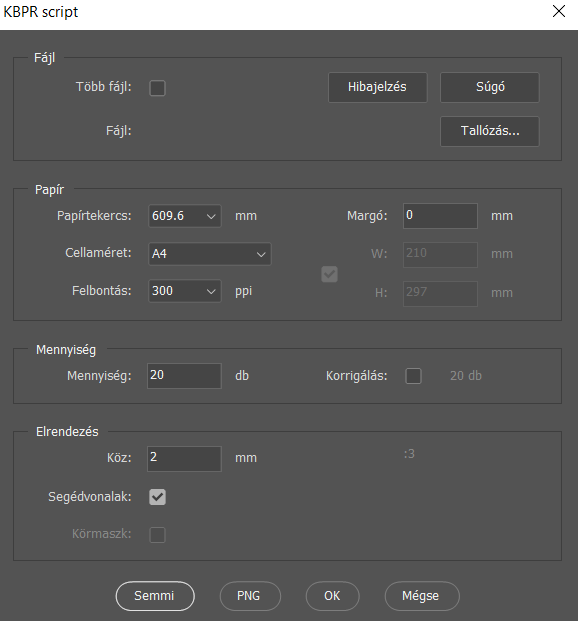
\includegraphics[width=\textwidth]{figures/script_showcase.png}
    \label{fig:old_ui}
    \caption{A kör által Photoshop script felhasználói felülete}
\end{figure}